\chapter{Implementation}
\label{cha:implementation}
In this chapter, we describe how we implemented the simulation. First, section~\ref{sec:components} presents the various components we developed by describing what their task is, what we noticed during the implementation and why we implemented it this way. \textcolor{red}{module dependencies extra or in modules?} In section~\ref{sec:module_dependencies}, we describe the dependencies and interaction between the modules we developed. Section~\ref{sec:imp_communication} covers the implementation of the communication between Fawkes and Gazebo and between multiple robots we want to simulate. In section~\ref{sec:agent_improvements}, we present the improvements for the multi-agent system we implemented during the thesis.

\section{Components}
\label{sec:components}
\subsection{Gazebo Models}
\begin{figure}
\centering
\begin{subfigure}[b]{0.48\textwidth}
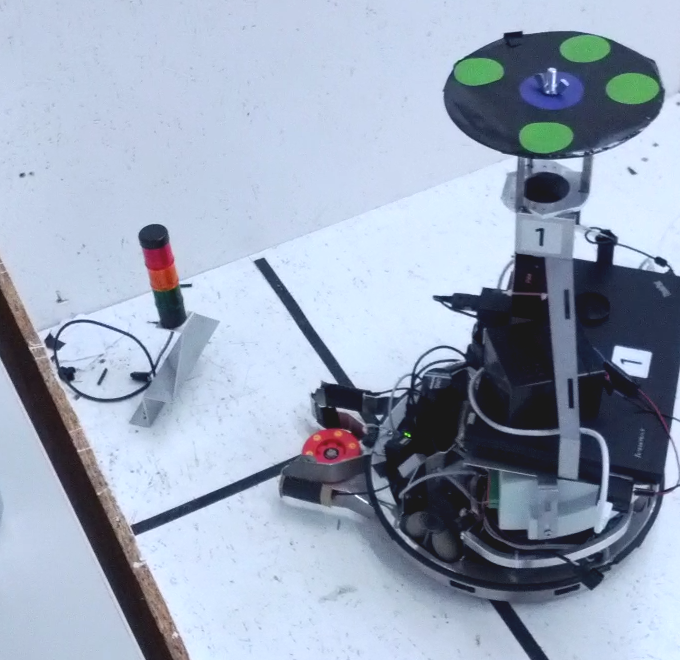
\includegraphics[width=\textwidth]{pics/llsf_real}
\caption{A Robotino delivers a puck to a recycling machine.}
\label{fig:comparison_real}
\end{subfigure}
\begin{subfigure}[b]{0.48\textwidth}
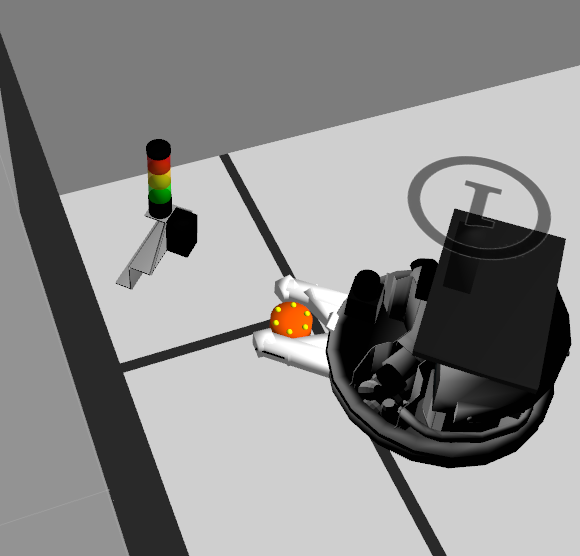
\includegraphics[width=\textwidth]{pics/llsf_sim}
\caption{The same situation in the Gazebo~simulation}
\label{fig:comparison_sim}
\end{subfigure}
\caption{Comparison of the real scene and the simulated scene in Gazebo}
\label{fig:comparison}
\end{figure}

In order to simulate the LLSF environment, we need to model all objects appearing in this domain. The models developed in this thesis are available at \url{https://github.com/zwilling/llsf-models.git}. Here, we present our simulation models and why we modeled them this way. Figure~\ref{fig:comparison} shows a comparison between a real LLSF scene and the same scene in the simulation. In this comparison, the most important objects of the simulation can be seen. In the following, we describe each model in detail:\\
\textbf{LLSF Field:} The model of the LLSF field has a rather simple structure. It consists of a ground plate and four side walls. For the visual appearance and possible future changes, the field has a visual representation with lines and colored areas just as on the real field. The machines are not realized as a component of the field and are attached to the field in the description of the simulation world.\\
\textbf{Machine:} The model of the machines matches the real machines structurally. Though, it is challenging to represent the lamps consisting of colored Plexiglas and a LED \textcolor{red}{abbreviation?} inside. We decided to use simple colored cylinders in the simulation. If the lamp is turned off, we use a dark and slightly transparent color and, if the light is turned on, we use a a bright color. This looks reasonable in the simulation and the images from the simulation are sufficient for our vision plugin which determines the lamp state of the machines. The vision plugin measures the brightness at the position where it expects the machine-lamp to be and it even was not necessary to change brightness thresholds. In Figure~\ref{fig:comparison_real}, the black RFID box in front of the machine is missing because we currently do not have the RFID readers.\\
\textbf{Puck:} The visual appearance of the puck model can be seen in Figure~\ref{fig:comparison_sim}. Physically, they are represented by a single cylinder. The difficult part was to find good friction parameters for the surface of the cylinder. On the one hand, it should be easy to slide the puck across the floor. On the other hand, the puck should stay inside the gripper of the Robotino when the Robotino turns. If the friction parameters are too small, the pucks move outside the gripper while turning because of the centrifugal force. \textcolor{red}{mention other solution?}\\
\textbf{Robotino:} The model of the Robotino is the most complex model because it holds different sensors, the casing and the puck gripper. It is also the most important one because it represents the robot we want to simulate. The major visual difference between real world and simulation is caused by the missing framework on top of the Robotino and the visual appearance of the puck gripper. Both is not important because we do net detect other Robotinos with a camera. We detect them with the laser sensor. Therefore and because of the manipulation with the gripper, the physical representation is more important. \textcolor{red}{collisions picture?} The physical model of the Robotino is composed of the gripper and two cylinders, one on the ground to represent the basic circle of the Robotino and one on laser and machine height. The cylinder on laser height is smaller and shifted back so that it does not block the laser sensor of the same Robotino and it fits better to the real shape. The gripper in the simulation has a similar shape than the real one. We needed to assign higher friction parameters to the inside of the gripper than to the outside because in reality the puck slides into the gripper if the front side of the gripper and stays in the gripper while turning. Because we were not able to simulate this with a single set of friction parameters, we modeled an additional geometry for the inside of the gripper with higher friction parameters. Originally, we intended to add wheels to the physical design for the final version. However, the omni-directional wheels caused an abnormal physical behavior in the simulation. The wheels irregularly bounced on the ground because of gravity and collision. Because we could not solve this problem in an arguable time and there is no important advantage, we decided to stay at the simple model without wheels. We only loose the possibility to physically simulate the odometry with its error. Therefore we introduced an artificially odometry error in the Gazebo plugin for the Robotino. \textcolor{red}{friction, setvel?}\\
\textbf{Simulation World:} The world file combines the developed models to an LLSF environment. Our world consists of the LLSF field, 16 machines with configurable orientation, 20 pucks and three Robotinos.\\


\subsection{Gazebo Plugins}
plugins for robot and worlds consisting of smaller reusable modules \textcolor{red}{refactoring necessary}
\textbf{World Plugin}
\\
\textbf{Robotino Plugin}
\\
\textbf{Native Plugins}


\subsection{Fawkes Plugins}
The Fawkes plugins developed in this thesis provide access to the simulation in Fawkes. In order to identify plugins for the Gazebo simulation quickly, we named them with the prefix \textit{Gazsim}. We divided the plugins into two groups. The first group of plugins generally cover the access to the Gazebo simulation, sensors and the Robotino robot without limitation to a specific domain or task. All these plugins can be found in the simulation branch of the Fawkes repository\footnote{http://git.fawkesrobotics.org/fawkes.git}. The second group of plugins are needed for the simulation of the LLSF environment. They can be found in our LLSF repository\footnote{http://git.fawkesrobotics.org/fawkes-robotino.git} which includes the general Fawkes repository. The access to the LLSF repository currently is limited because it contains new code we want to take advantage of in the LLSF competition.

\subsubsection{Common Gazebo and Robotino Plugins}
\textbf{Gazebo:} The plugin called \textit{Gazebo} provides general access to the Gazebo Transport API which is needed to communicate with the simulator. Therefore, it provides a Fawkes aspect also called \textit{Gazebo}. After connection to the Gazebo simulator, the aspect gives access to two communication nodes. One node is responsible for the communication with the simulated robot Fawkes should control and has to be initialized with the name of the robot in the simulation. The other node is responsible for the communication with the simulation world and therefore used for robot independent information environment information. It is also possible to spawn new models and visuals through this node. This is useful for controlling of the simulation and visualizing tasks to show, for example, the robot intention. \textcolor{red}{bei klingen noch nicht multi-roboter faehig?}
\\
\textbf{Gazsim-Robotino:}
The \textit{Gazsim-Robotino} plugin exchanges the Robotino plugin which connects Fawkes with the hardware of the Robotino robot. Therefore our plugin provides the same interfaces as the original plugin. The original plugin provides motor and sensor features, each with an own interface. Because both are combined in the original plugin, we also combine these two features in the simulation plugin. However, we developed separate modules for these two features to improve re-usability. The module responsible for the motor sends the wished motor movement to Gazebo and receives the position of the robot in the simulation to compute the odometry. Because sending many Protobuf messages has been found to be computationally costly, we only send messages if he wished movement has changed. Here we also introduced an error to the odometry which occurs more strong when the speed changes quickly. As in reality, the odometry also changes if the robot drives against an obstacle and does not change it's position. \textcolor{red}{important because driving against machine?} The module responsible for the sensors of the Robotino receives information from the simulated gyroscope and distance sensors of the Robotino.
\\
\textbf{Gazsim-Laser:}
The \textit{Gazsim-Laser} plugin exchanges the laser plugin and provides data from a simulated laser range sensor. The plugin converts received data into the in Fawkes used format and writes it into the laser-interface. \textcolor{red}{difference 5m-Nan?}
\\
\textbf{Gazsim-Localization:}
The plugin called \textit{Gazsim-Localization} receives the position of the robot in the simulation and publishes this information in the corresponding interface. Normally, this information is provided by plugins, such as amcl (Adaptive Monte Carlo Localization). Therefore this plugin operates on a higher level of abstraction. It uses ground truth information to allow testing high level components without error in the localization. 
\\
\textbf{Gazsim-Webcam:}
The \textit{Gazsim-Webcam} plugin receives a camera image from the gazebo simulation. It converts the received image from RGB\textcolor{red}{explain abbrv?}, which is used in Gazebo, into YUV\textcolor{red}{explain abbrv?}, which is used in Fawkes, and writes the image to a shared memory buffer. Unlike in other simulation plugins, there is no interface because vision plugins can directly load a camera through Fawkes tools. However, it is possible to load a shared memory image in the same way as a real camera. The vision plugin just has to be configured to use an other camera-identification string. We identify the shared memory images with the robot name as prefix because multiple Fawkes instances use the same set of shared memory images. Otherwise, there would be one shared memory image which alternately shows camera images from different robots.
\\
\textbf{Gazsim-Timesource:}
The \textit{Gazsim-Timesource} plugin provides the simulation time in Fawkes. This is important to avoid timing problems that occur if the computer is not able to run the simulation at real-time. Furthermore it allows to run the simulation faster than real time to speed up the testing process. The plugin replaces the default time-source in Fawkes. To provide a precise time avoid bad performance because of many synchronization messages, we decided to estimate the simulation time between two received time messages from Gazebo by using the current simulation speed and the real time passed since the last time synchronization message. To guarantee a monotonous time, we do not set the time in Fawkes back if the simulation has slowed down between two time synchronization messages. The error can create a error in time and is more acceptable than a worse performance with many  messages and a frozen time between two messages.
\textcolor{red}{measurement for created time error}\\
\textbf{Gazsim-Comm:}
The \textit{Gazsim-Comm} plugin simulates the communication between multiple Fawkes instances without using Gazebo. It runs on a separate Fawkes instance which does not control a simulated robot and acts similar to a hub. It uses a set of peer-to-peer connections to the different Fawkes instances and forwards broadcast messages from one peer to all other peers. This solves the problem that usually the different Fawkes instances communicate on the same ports which is not directly possible if the instances run on the same computer. We preferred this approach over others because also want to simulate communication over a bad wireless network. This is an important problem we want to simulate because during the RoboCup competition the wireless network usually is over-crowded. The package loss is simulated by the plugin by setting the likelihood for messages to be dropped before forwarding.
\\
\textbf{Gazsim-Vis-Localization:}
The \textit{Gazsim-Vis-Localization} plugin visualizes the localization of a robot in the simulation. It spawns a label which identifies the robot with an arrow which indicates the orientation of the robot above the position where the robot believes to be. The visualization is only visible from above so that the robot can not the label in the simulation. This visualization is very useful during testing because a wrong localization is one of the most common reasons for misbehaving of the robot. Without this visualization in the simulation, it would be time-consuming to check the localization of multiple robots because it would be necessary to look into a separate Rviz for each robot. Furthermore, the visualization can be used to indicate the localization of the robots in a reconstruction of an automated simulation run.
\\


\subsubsection{LLSF specific Plugins}
\textbf{Gazsim-Light-Front:}
The plugin \textit{Gazsim-Light-Front} exchanges the vision plugin \textit{Light-Front} which determines the light state of machines by using a webcam. Light-Front uses the laser-cluster detection to know where to look for the machine light in the camera picture. Gazsim-Light-Front also uses laser-cluster results and the positions of the machines to determine on which machine the Robotino is looking at. If there is a machine near the position returned by the laser-cluster the plugin determines the light state by using the last message received from Gazebo. The plugin also writes the visibility history, which indicates how long the vision result is stable, and the ready flag, which indicates if the plugin beliefs it has correctly determined the light state. This plugin also simulates on a higher level of abstraction and provides ground truth information about the machine light states. This is useful for testing the agent because a wrongly detected light can have a crucial impact on the performance of the system.
\\
\textbf{Gazsim-Puck-Detection:}
The plugin \textit{Gazsim-Puck-Detection} replaces the plugin \textit{Omnivision-Pucks} which finds pucks by using the omni-directional camera. Gazsim-Puck-Detection receives the positions of the robot and the pucks from Gazebo and writes the position of the pucks relative to the robot into the corresponding interface. A puck is only recognized if it is in a certain area around the robot. The maximal distance is similar to the real range in which Omnivision-Pucks can detect pucks. Here we also have a plugin with high level abstraction. Omnivision-Pucks sometimes has problems with two pucks lying next to each other because it can interpret them as one puck with the center between both pucks. This can cause problems when trying to grab a puck and therefore providing ground truth data about the puck positions can be useful for testing.
\\
\textbf{Gazsim-LLSFrbcomm:}
The plugin \textit{Gazebo-LLSFrbcomm} connects the LLSF Refbox with the Gazebo simulation. It connects to the Refbox as a client because only clients receive information about the machine light status. On the one hand it sends received information about the machine light status to Gazebo via Protobuf messages. On the other hand it receives messages from Gazebo about pucks placed or removed under RFID readers of machines and sends this information as a client to the Refbox. We did not implement the connection to the Refbox directly in the simulation because Fawkes already provides a simple way for the connection and we do not want to duplicate the code used there. This plugin also sends the simulation time to the Refbox. \textcolor{red}{important bla?} In this context we modified the Refbox to use the simulation time messages similar as the Gazsim-Timesource plugin. Similar as Gazsim-Comm, the plugin can run in a robot independent Fawkes instance.
\\
\textbf{Gazsim-LLSF-Control:}
The plugin \textit{Gazsim-LLSF-Control} works in combination with the automation scripts. It waits until the Refbox announces that the game is over and then stops the simulation run. The automation script recognizes that the simulation stopped and can start a new run. This plugin also can be started in a robot independent Fawkes instance.
\\
\textbf{Gazsim-LLSF-Statistics:}
The plugin \textit{Gazsim-LLSF-Statistics} keeps statistics about the result of automated simulation runs. For example it keeps track of the amount of points scored in the several phases, the types of pucks being produced and the used configuration. When the game is over, the plugin writes these statistics to MongoDB. The statistics collected in a simulation run are inserted as a single document in the collection which includes all simulation runs of the schedule initiated with the automation script.



\subsection{Automation Scripts}
There are two major reasons why we decided to develop scripts to automate starting the simulation. On the one hand, a full LLSF simulation with three simulated robots requires a large amount of running programs. It is necessary to start Gazebo, the Refbox, a Fawkes instance for robot independent plugins and for each robot a separate Roscore, Movebase and Fawkes instance. Starting all programs with the required parameters is time consuming and can be automated. On the other hand, we need an automated startup if we want to run multiple simulation runs. This is usefull to get an overview of the average system performance and to compare different strategies and configurations. Therefore it should be possible to let the simulation run 20 times with different configurations over night.\\
We implemented the automation scripts as simple bash scripts because they are powerful and easy to use and extend. There are two main automation scripts called \textit{gazsim.bash} and \textit{gazsim-schedule.bash}. The script gazsim.bash can start or stop a simulation and has several options. It is possible to start the simulation with a specific configuration and amount of robots. The simulation can also be started in a headless mode\footnote{In the headless mode, Gazebo runs without a graphical user interface. This can save computation time. Although there is no visualization for the user, all visual sensors are still simulated.}. It is also possible to determine if the simulation starts with ROS, recording, statistics and which level of abstraction should be used. With the script gazsim-schedule.bash, multiple simulation runs can be scheduled. It is possible to define a set of configurations, which should be compared, the amount of simulation runs for each configuration and the level of abstraction.

\section{Module Dependencies}
\label{sec:module_dependencies}


\section{Communication}
\label{sec:imp_communication}


\section{Agent Improvements}
\label{sec:agent_improvements}
The main taks we want to use our simulator for is the improvement of our multi-robot system. Therefore improving our agent in this thesis is doubly important because we need it anyway and it is neccessary to evaluate how useful our simulator is for the development of a multi-robot system. In the following we present the three major improvements we made during this thesis. These improvements are not independent from each other because whe combine them to improve the system even further. In addition, we also made several minor improvements. We mention these during this section and the evaluation chapter, when we present some of the problems found with the simulation.


\subsection{Using Three Agents}
Before the thesis, we used only two of three usable robots in the competition. Because we want to maximize our performance in LLSF, we have to use all three robots. In this thesis, we extend our current role based approach to work with three robots. On the one hand, we introduce new roles which can be easily allocated to the three robots. On the other hand, we try how the current roles work with three robots and where the limitations are. A part of this is covered in the evaluation chapter.\\
First we introduced two new roles by splitting the old P1P2-role which produces P1 or P2 depending on what lets the P3 agent more space. Now we have a P1-role and a P2-role, which produce only P1 or respectively P2. Both roles use a disjoint set of machines to avoid conflicts while producing intermediate products. To coordinate the use of resources shared by multiple robots, such as the delivery machines, we use the already existing locking mechanism which scales well with an additional robot. Therefore, we can also assing multiple robots to the P3-role because there is no context information needed to produce a P3. Everytime a robot receives a lock of the T5 machine, which produces P3, the robot can bring a new resource puck to produce a P3. Actually, assigning multiple robots to the P3-role seems to be a good idea because P3 is often highly demanded and producing P3 provides simple and quick points. There also are adjustment we have to make to use three robots in the exploration phase. The three agents have to manage which robot explores which machine. Our current approach defines a circular path passing all machines. Each agents start at a spezified machine and explores all unknown machines along this path and can pass already explored machines and machines that are blocked by other agents. To use this approach with three agents, we sepatated the start machine from the role in the production phase and introduced a new set of starting machines.

\subsection{Recycling}
An other opportunity we were not able to use before the thesis is recycling. Recycling of consumed pucks can provide quick points because each recycled puck gives five points and takes only around to seconds to produce on a recycling machine. When using three robots it is also useful to reduce over-crowding of the insertion area where robots usually get new resource pucks from. The implementation of the recycling took two basic steps. First, we implemented neccessary skills of the robot to grep a consumed puck lying next to a machine and to use a recycling machine. We have to use an modified method to use recycling machines because our usual one for normal machines does not work in the corner of the field. Here, the simulation already revealed a problem we did not know about before. The two digital optical sensors which we use to check if the robot stands directly before the machine does not work in the corner of the field. The sensor triggers if there is an obstacle in a certain range in front of the sensor and if the robot stands near a recycling machine, the sensor already triggers because the wall of the field is in this range. Because we can decrease this range in the simulation, it is possible to test and continue the rest of the development neccessary for recycling. This is not so easily possible in reality. The second part of the implementation was including recycling in the agent. Therefore the agent has to keep in mind where consumed pucks are and to know how and where to recycle them. We also implemented the possibility to configure when to do the recycling. Currently, the agent can recycle whenever it is possible and it needs a new S0 or when the production of a P1 or P2 is finished and there is no risk on loosing the points for the product caused by a failure during recycling. We decided to introduce no recycling role because it would be less effective than doing recycling as an alterative way to get a new S0. The reason is that an agent with a recycling-only role would drop the new resource puck which could be used for a production step.

\subsection{Dynamic Role Change}
Our current static role based approach has the downside that the role allocation can not be adapted to the current situation. In some situations, there are roles which are significantly less useful than other roles. For example, assigning a P1-role to a robot makes no sense if there are no more P1 pucks ordered. Therefore, the robot should better produce P2 or P3 pucks. To be able to adapt the role allocation to the current situation, we introduced a dynamic role change. This dynamic role change is based on a set of rules which define under which circumstances a role is changed into an other role.

dynamic role switch: no more products ordered, \cite{dynamic_role_assignment}


